\documentclass[10pt,oneside]{article}
\usepackage[T1]{fontenc}
\usepackage[utf8]{inputenc}
%\usepackage[latin1]{inputenc}
\DeclareUnicodeCharacter{00A0}{ }
% \usepackage{lmodern}
%\usepackage[adobe-utopia,uppercase=upright,greeklowercase=upright]{mathdesign}
\usepackage[adobe-utopia]{mathdesign}
%\usepackage{minionpro}
% \usepackage{pifont}
% \usepackage{amssymb}
\usepackage{amsmath}
\usepackage[francais]{babel}
% \usepackage[francais]{varioref}
\usepackage[dvips]{graphicx}
\usepackage{here}
\usepackage{framed}
\usepackage[normalem]{ulem}
\usepackage{fancyhdr}
\usepackage{titlesec}
\usepackage{vmargin}
\usepackage{longtable}

\usepackage{amsmath}

\usepackage{ifthen}
%\usepackage[•]{caption}

%\usepackage{epsfig}
\usepackage{subfig}

\usepackage{multirow}
\usepackage{multicol} % Portions de texte en colonnes
\usepackage{flafter}%floatants après la référence



\usepackage{color}
\usepackage{colortbl}


\definecolor{gris25}{gray}{0.75}
\definecolor{bleu}{RGB}{18,33,98}
\definecolor{bleuf}{RGB}{42,94,171}
\definecolor{bleuc}{RGB}{231,239,247}
\definecolor{rougef}{RGB}{185,18,27}
\definecolor{rougec}{RGB}{255,230,231}
\definecolor{vertf}{RGB}{103,126,82}
\definecolor{vertc}{RGB}{220,255,191}
\definecolor{violetf}{RGB}{112,48,160}
\definecolor{violetc}{RGB}{230,224,236}
\definecolor{jaunec}{RGB}{220,255,191}


\newenvironment{corrige}[1][\hsize]%
{%
    \def\FrameCommand
    {%
\rotatebox{90}{\textit{\textsf{Correction}}} 
        {\color{violetf}\vrule width 3pt}%
        \hspace{0pt}%must no space.
        \fboxsep=\FrameSep\colorbox{violetc}%
    }%
    \MakeFramed{\hsize#1\advance\hsize-\width\FrameRestore}%
}%
{\endMakeFramed}%



\newenvironment{sci}[1][\hsize]%
{%
    \def\FrameCommand%
    {%
%\rotatebox{90}{\textit{\textsf{Scilab}}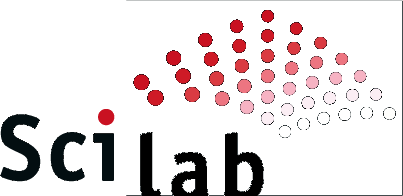
\includegraphics[height=.8cm]{png/logo_scilab}} 
\rotatebox{90}{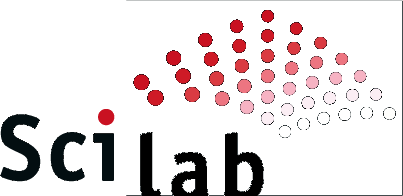
\includegraphics[height=.6cm]{png/logo_scilab}} 
        {\color{violetf}\vrule width 3pt}%
        \hspace{0pt}%must no space.
        \fboxsep=\FrameSep\colorbox{violetc}%
    }%
    \MakeFramed{\hsize #1 \advance\hsize-\width\FrameRestore}%
}%
{\endMakeFramed}%

\newenvironment{pseudo}[1][\hsize]%
{%
    \def\FrameCommand%
    {%
\rotatebox{90}{\textit{\textsf{Pseudo Code}}} 
        {\color{violetf}\vrule width 3pt}%
        \hspace{0pt}%must no space.
        \fboxsep=\FrameSep\colorbox{violetc}%
    }%
    \MakeFramed{\hsize #1 \advance\hsize-\width\FrameRestore}%
}%
{\endMakeFramed}%

\newenvironment{py}[1][\hsize]%
{%prof
    \def\FrameCommand%
    {%
%\rotatebox{90}{\textit{\textsf{Python}}} 
\rotatebox{90}{
\includegraphics[height=.6cm]{png/logo_python}} 
        {\color{violetf}\vrule width 3pt}%
        \hspace{0pt}%must no space.
        \fboxsep=\FrameSep\colorbox{violetc}%
    }%
    \MakeFramed{\hsize #1 \advance\hsize-\width\FrameRestore}%
}%
{\endMakeFramed}%


\newenvironment{term}[1][\hsize]%
{%
    \def\FrameCommand%
    {%
\rotatebox{90}{\textit{\textsf{Terminal}}} 
        {\color{violetf}\vrule width 3pt}%
        \hspace{0pt}%must no space.
        \fboxsep=\FrameSep\colorbox{violetc}%
    }%
    \MakeFramed{\hsize #1 \advance\hsize-\width\FrameRestore}%
}%
{\endMakeFramed}%


\newenvironment{rem}[1][\hsize]%
{%
    \def\FrameCommand
    {%
\rotatebox{90}{\textit{\textsf{Remarque}}} 
        {\color{bleuf}\vrule width 3pt}%
        \hspace{0pt}%must no space.
        \fboxsep=\FrameSep\colorbox{bleuc}%
    }%
    \MakeFramed{\hsize#1\advance\hsize-\width\FrameRestore}%
}%
{\endMakeFramed}%


\newenvironment{savoir}[1][\hsize]%
{%
    \def\FrameCommand
    {%
\rotatebox{90}{\textit{\textsf{Savoir}}} 
        {\color{bleuf}\vrule width 3pt}%
        \hspace{0pt}%must no space.
        \fboxsep=\FrameSep\colorbox{bleuc}%
    }%
    \MakeFramed{\hsize#1\advance\hsize-\width\FrameRestore}%
}%
{\endMakeFramed}%

\newenvironment{Objectif}[1][\hsize]%
{%
    \def\FrameCommand
    {%
\rotatebox{90}{\textit{\textsf{Objectif}}} 
        {\color{bleuf}\vrule width 3pt}%
        \hspace{0pt}%must no space.
        \fboxsep=\FrameSep\colorbox{bleuc}%
    }%
    \MakeFramed{\hsize#1\advance\hsize-\width\FrameRestore}%
}%
{\endMakeFramed}%

\newenvironment{prob}[1][\hsize]%prof
{%
    \def\FrameCommand%
    {%
\rotatebox{90}{\textit{\textsf{ Problématique}}} 
        {\color{rougef}\vrule width 3pt}%
        \hspace{0pt}%must no space.
        \fboxsep=\FrameSep\colorbox{rougec}%
    }%
    \MakeFramed{\hsize#1\advance\hsize-\width\FrameRestore}%
}%
{\endMakeFramed}%

\newenvironment{obj}[1][\hsize]%
{%
    \def\FrameCommand%
    {%
\rotatebox{90}{\textit{\textsf{ $\;$}}} 
        {\color{rougef}\vrule width 3pt}%
        \hspace{0pt}%must no space.
        \fboxsep=\FrameSep\colorbox{rougec}%
    }%
    \MakeFramed{\hsize#1\advance\hsize-\width\FrameRestore}%
}%
{\endMakeFramed}%

\newenvironment{defi}[1][\hsize]%
{%
    \def\FrameCommand%
    {%
\rotatebox{90}{\textit{\textsf{Définition\\}}} 
        {\color{bleuf}\vrule width 3pt}%
        \hspace{0pt}%must no space.
        \fboxsep=\FrameSep\colorbox{bleuc}%
    }%
    \MakeFramed{\hsize#1\advance\hsize-\width\FrameRestore}%
}%
{\endMakeFramed}%


\newenvironment{demo}[1][\hsize]%
{%
    \def\FrameCommand%
    {%
\rotatebox{90}{\textit{\textsf{Démonstration\\}}} 
        {\color{bleuf}\vrule width 3pt}%
        \hspace{0pt}%must no space.
        \fboxsep=\FrameSep\colorbox{bleuc}%
    }%
    \MakeFramed{\hsize#1\advance\hsize-\width\FrameRestore}%
}%
{\endMakeFramed}%


\newenvironment{hypo}[1][\hsize]%
{%
    \def\FrameCommand%
    {%
\rotatebox{90}{\textit{\textsf{Hypothèse\\}}} 
        {\color{bleuf}\vrule width 3pt}%
        \hspace{0pt}%must no space.
        \fboxsep=\FrameSep\colorbox{bleuc}%
    }%
    \MakeFramed{\hsize#1\advance\hsize-\width\FrameRestore}%
}%
{\endMakeFramed}%


\newenvironment{prop}[1][\hsize]%
{%
    \def\FrameCommand%
    {%
\rotatebox{90}{\textit{\textsf{Propriété\\}}} 
        {\color{bleuf}\vrule width 3pt}%
        \hspace{0pt}%must no space.
        \fboxsep=\FrameSep\colorbox{bleuc}%
    }%
    \MakeFramed{\hsize#1\advance\hsize-\width\FrameRestore}%
}%
{\endMakeFramed}%

\newenvironment{props}[1][\hsize]%
{%
    \def\FrameCommand%
    {%
\rotatebox{90}{\textit{\textsf{Propriétés\\}}} 
        {\color{bleuf}\vrule width 3pt}%
        \hspace{0pt}%must no space.
        \fboxsep=\FrameSep\colorbox{bleuc}%
    }%
    \MakeFramed{\hsize#1\advance\hsize-\width\FrameRestore}%
}%
{\endMakeFramed}%

\newenvironment{exemple}[1][\hsize]%
{%
    \def\FrameCommand%
    {%
\rotatebox{90}{\textit{\textsf{Exemple\\}}} 
        {\color{vertf}\vrule width 3pt}%
        \hspace{0pt}%must no space.
        \fboxsep=\FrameSep\colorbox{vertc}%
    }%
    \MakeFramed{\hsize#1\advance\hsize-\width\FrameRestore}%
}%
{\endMakeFramed}%

\newenvironment{exercice}[1][\hsize]%
{%
    \def\FrameCommand%
    {%
\rotatebox{90}{\textit{\textsf{Exercice\\}}} 
        {\color{vertf}\vrule width 3pt}%
        \hspace{0pt}%must no space.
        \fboxsep=\FrameSep\colorbox{vertc}%
    }%
    \MakeFramed{\hsize#1\advance\hsize-\width\FrameRestore}%
}%
{\endMakeFramed}%

\newenvironment{Support}[1][\hsize]%
{%
    \def\FrameCommand%
    {%
\rotatebox{90}{\textit{\textsf{Support de cours\\}}} 
        {\color{vertf}\vrule width 3pt}%
        \hspace{0pt}%must no space.
        \fboxsep=\FrameSep\colorbox{jaunec}%
    }%
    \MakeFramed{\hsize#1\advance\hsize-\width\FrameRestore}%
}%
{\endMakeFramed}%

\newenvironment{resultat}[1][\hsize]%
{%
    \def\FrameCommand%
    {%
\rotatebox{90}{\textit{\textsf{Résultat\\}}} 
        {\color{rougef}\vrule width 3pt}%
        \hspace{0pt}%must no space.
        \fboxsep=\FrameSep\colorbox{rougec}%
    }%
    \MakeFramed{\hsize#1\advance\hsize-\width\FrameRestore}%
}%
{\endMakeFramed}%

\newenvironment{methode}[1][\hsize]%
{%
    \def\FrameCommand%
    {%
\rotatebox{90}{\textit{\textsf{Méthode\\}}} 
        {\color{rougef}\vrule width 3pt}%
        \hspace{0pt}%must no space.
        \fboxsep=\FrameSep\colorbox{rougec}%
    }%
    \MakeFramed{\hsize#1\advance\hsize-\width\FrameRestore}%
}%
{\endMakeFramed}%

\newenvironment{theo}[1][\hsize]%
{%
    \def\FrameCommand%
    {%
\rotatebox{90}{\textit{\textsf{Théorème\\}}} 
        {\color{rougef}\vrule width 3pt}%
        \hspace{0pt}%must no space.
        \fboxsep=\FrameSep\colorbox{rougec}%
    }%
    \MakeFramed{\hsize#1\advance\hsize-\width\FrameRestore}%
}%
{\endMakeFramed}%

\newenvironment{warn}[1][\hsize]%
{%
    \def\FrameCommand%
    {%
\rotatebox{90}{\textit{\textsf{Attention\\}}} 
        {\color{rougef}\vrule width 3pt}%
        \hspace{0pt}%must no space.
        \fboxsep=\FrameSep\colorbox{rougec}%
    }%
    \MakeFramed{\hsize#1\advance\hsize-\width\FrameRestore}%
}%
{\endMakeFramed}%

% \usepackage{pstricks}
%\usepackage{minitoc}
% \setcounter{minitocdepth}{4}

\setcounter{tocdepth}{2}

% \mtcselectlanguage{french} 

%\usepackage{draftcopy}% "Brouillon"
% \usepackage{floatflt}
\usepackage{psfrag}
%\usepackage{listings} % Permet d'insérer du code de programmation
\renewcommand{\baselinestretch}{1.2}

% Changer la numérotation des figures :
% ------------------------------------
% \makeatletter
% \renewcommand{\thefigure}{\ifnum \c@section>\z@ \thesection.\fi
%  \@arabic\c@figure}
% \@addtoreset{figure}{section}
% \makeatother
 


%%%%%%%%%%%%
% Définition des vecteurs %
%%%%%%%%%%%%
 \newcommand{\vect}[1]{\overrightarrow{#1}}

%%%%%%%%%%%%
% Définition des torseusr %
%%%%%%%%%%%%

 \newcommand{\torseur}[1]{%
\left\{{#1}\right\}
}

\newcommand{\torseurcin}[3]{%
\left\{\mathcal{#1} \left(#2/#3 \right) \right\}
}

\newcommand{\torseurstat}[3]{%
\left\{\mathcal{#1} \left(#2\rightarrow #3 \right) \right\}
}

 \newcommand{\torseurc}[8]{%
%\left\{#1 \right\}=
\left\{
{#1}
\right\}
 = 
\left\{%
\begin{array}{cc}%
{#2} & {#5}\\%
{#3} & {#6}\\%
{#4} & {#7}\\%
\end{array}%
\right\}_{#8}%
}

 \newcommand{\torseurcol}[7]{
\left\{%
\begin{array}{cc}%
{#1} & {#4}\\%
{#2} & {#5}\\%
{#3} & {#6}\\%
\end{array}%
\right\}_{#7}%
}

 \newcommand{\torseurl}[3]{%
%\left\{\mathcal{#1}\right\}_{#2}=%
\left\{%
\begin{array}{l}%
{#1} \\%
{#2} %
\end{array}%
\right\}_{#3}%
}

 \newcommand{\vectv}[3]{%
\vect{V\left( {#1} \in {#2}/{#3}\right)}
}


\newcommand{\vectf}[2]{%
\vect{R\left( {#1} \rightarrow {#2}\right)}
}

\newcommand{\vectm}[3]{%
\vect{\mathcal{M}\left( {#1}, {#2} \rightarrow {#3}\right)}
}


 \newcommand{\vectg}[3]{%
\vect{\Gamma \left( {#1} \in {#2}/{#3}\right)}
}

 \newcommand{\vecto}[2]{%
\vect{\Omega\left( {#1}/{#2}\right)}
}
% }$$\left\{\mathcal{#1} \right\}_{#2} =%
% \left\{%
% \begin{array}{c}%
%  #3 \\%
%  #4 %
% \end{array}%
% \right\}_{#5}}

%  ------------------------------------------
% | Modification du formatage des sections : | 
%  ------------------------------------------

% Grands titres :
% ---------------

\newcommand{\titre}[1]{%
\begin{center}
      \bigskip
      \rule{\textwidth}{1pt}
      \par\vspace{0.1cm}
      
      \textbf{\large #1}
      \par\rule{\textwidth}{1pt}
    \end{center}
    \bigskip
  }

% Supprime le numéro du chapitre dans la numérotation des sections:
% -----------------------------------------------------------------
\makeatletter
\renewcommand{\thesection}{\@arabic\c@section}
\makeatother


% \titleformat{\chapter}[display]
% {\normalfont\Large\filcenter}
% {}
% {1pc}
% {\titlerule[1pt]
%   \vspace{1pc}%
%   \Huge}[\vspace{1ex}%
% \titlerule]


%%%% Chapitres Comme PY Pechard %%%%%%%%%
% numéro du chapitre
\DeclareFixedFont{\chapnumfont}{OT1}{phv}{b}{n}{80pt}
% pour le mot « Chapitre »
\DeclareFixedFont{\chapchapfont}{OT1}{phv}{m}{it}{40pt}
% pour le titre
\DeclareFixedFont{\chaptitfont}{T1}{phv}{b}{n}{25pt}

\definecolor{gris}{gray}{0.75}
\titleformat{\chapter}[display]%
	{\sffamily}%
	{\filleft\chapchapfont\color{gris}\chaptertitlename\
	\\
	\vspace{12pt}
	\chapnumfont\thechapter}%
	{16pt}%
	{\filleft\chaptitfont}%
	[\vspace{6pt}\titlerule\titlerule\titlerule]

%%%%  Fin Chapitres Comme PY Pechard %%%%%%%%%


% Section, subsection, subsubsection sans serifs :
% % ----------------------------------------------

% \makeatletter
% \renewcommand{\section}{\@startsection{section}{0}{0mm}%
% {\baselineskip}{.3\baselineskip}%
% {\normalfont\sffamily\Large\textbf}}%
% \makeatother

\makeatletter
\renewcommand{\@seccntformat}[1]{{\textcolor{bleu}{\csname
the#1\endcsname}\hspace{0.5em}}}
\makeatother

\makeatletter
\renewcommand{\section}{\@startsection{section}{1}{\z@}%
                       {-4ex \@plus -1ex \@minus -.4ex}%
                       {1ex \@plus.2ex }%
                       {\normalfont\Large\sffamily\bfseries}}%
\makeatother
 
\makeatletter
\renewcommand{\subsection}{\@startsection {subsection}{2}{\z@}
                          {-3ex \@plus -0.1ex \@minus -.4ex}%
                          {0.5ex \@plus.2ex }%
                          {\normalfont\large\sffamily\bfseries}}
\makeatother
 
\makeatletter
\renewcommand{\subsubsection}{\@startsection {subsubsection}{3}{\z@}
                          {-2ex \@plus -0.1ex \@minus -.2ex}%
                          {0.2ex \@plus.2ex }%
                          {\normalfont\large\sffamily\bfseries}}
\makeatother
 
\makeatletter             
\renewcommand{\paragraph}{\@startsection{paragraph}{4}{\z@}%
                                    {-2ex \@plus-.2ex \@minus .2ex}%
                                    {0.1ex}%               
{\normalfont\sffamily\bfseries}}
\makeatother
 



\makeatletter             
\renewcommand{\subparagraph}{\@startsection{subparagraph}{5}{\z@}%
                                    {-2ex \@plus-.2ex \@minus .2ex}%
                                    {0.1ex}%               
{\normalfont\bfseries Question }}
\makeatother
\renewcommand{\thesubparagraph}{\arabic{subparagraph}} 
\makeatletter

\setcounter{secnumdepth}{5}


%  --------
% | Marges |
%  --------


% \setmarginsrb{2.5cm}{1.5cm}{2.5cm}{2cm}{1cm}{1cm}{1cm}{1cm}
\setmarginsrb{1.5cm}{1cm}{1cm}{1.5cm}{1cm}{1cm}{1cm}{1cm}

% Changer les marges localement :
% -----------------------------
\newenvironment{changemargin}[2]{\begin{list}{}{%
\setlength{\topsep}{0pt}%
\setlength{\leftmargin}{0pt}%
\setlength{\rightmargin}{0pt}%
\setlength{\listparindent}{\parindent}%
\setlength{\itemindent}{\parindent}%
\setlength{\parsep}{0pt plus 1pt}%
\addtolength{\leftmargin}{#1}%
\addtolength{\rightmargin}{#2}%
}\item }{\end{list}}



\usepackage{pst-solides3d}
\usepackage{titletoc}
\titlecontents{chapter}[+3pc]
  {\addvspace{10pt}\sffamily\bfseries}
{\contentslabel[{\pscirclebox[fillstyle=solid,fillcolor=gray!25,
linecolor=gray!25,framesep=4pt]{\textcolor{white}{\thecontentslabel}}}]{2.5pc}}
  {}
  {\dotfill \normalfont\thecontentspage\ }

\titlecontents{section}[3pc]
  {\addvspace{2pt}\sffamily}
  {\contentslabel[\thecontentslabel]{1.8pc}}
  {}
  {\dotfill \normalfont\thecontentspage\ }

\titlecontents{subsection}[5pc]
  {\addvspace{2pt}\sffamily}
  {\contentslabel[\thecontentslabel]{1.8pc}}
  {}
  {\dotfill \normalfont\thecontentspage\ }

\titlecontents{subsubsection}[8pc]
  {\addvspace{2pt}\sffamily}
  {\contentslabel[\thecontentslabel]{3pc}}
  {}
  {\dotfill \normalfont\thecontentspage\ }
%{\;\titlerule\;\normalfont\thecontentspage\ }

\titlecontents{paragraph}[9pc]
  {\addvspace{2pt}\sffamily}
  {\contentslabel[\thecontentslabel]{3.5pc}}
  {}
  {\dotfill \normalfont\thecontentspage\ }

%pour avoir l indentation dans minipage
\newdimen\oldparindent\oldparindent=\parindent

\makeatletter
\def\@iiiminipage#1#2[#3]#4{%
  \noindent
  \leavevmode
  \@pboxswfalse
  \setlength\@tempdima{#4}%
  \def\@mpargs{{#1}{#2}[#3]{#4}}%
  \setbox\@tempboxa\vbox\bgroup
    \color@begingroup
      \hsize\@tempdima
      \textwidth\hsize \columnwidth\hsize
      \@parboxrestore
      \parindent=\oldparindent
      \def\@mpfn{mpfootnote}\def\thempfn{\thempfootnote}\c@mpfootnote\z@
      \let\@footnotetext\@mpfootnotetext
      \let\@listdepth\@mplistdepth \@mplistdepth\z@
      \@minipagerestore
      \@setminipage}
\makeatother

%Definition de la commande question
\newcounter{Qu}
\newcommand{\Question}[2][0]{
\ifthenelse{\equal{#1}{0}}                      %demande-t-on une minipage ?
{\medskip\noindent {\refstepcounter{Qu}\textbf{Q\theQu .\hspace{0,7mm}}#2}\ifshowanswers \else \smallskip \fi}  %non donc on balance le texte
{\ifshowanswers                                 %oui minipage en mode problem
\noindent {\refstepcounter{Qu}\textbf{Q\theQu .\hspace{0,7mm}}#2}    %mode solution
\else                                           %mode problem
\noindent\begin{minipage}{#1}\noindent {\refstepcounter{Qu}\textbf{Q\theQu .\hspace{0,7mm}}#2}\end{minipage}\smallskip
\fi }
}

\newcommand{\Questionpb}[2][0]{%le premier argument entre [] est par défaut à 0
\begin{onlyproblem}\Question[#1]{#2}\end{onlyproblem}
}

\newcommand{\Onlyproblem}[2][0]{%le premier argument entre [] est par défaut à 0
%si le 2e arguement est 0
\ifthenelse{\equal{#1}{0}}
%on demande un environnement pb classique
{\begin{onlyproblem}#2\end{onlyproblem}}
%sinon on demande à faire une minipage
{\begin{onlyproblem}\noindent\begin{minipage}{#1}\parskip2ex #2\end{minipage}\smallskip \end{onlyproblem} }
}

\newcounter{Sl}
\addtocounter{Sl}{+1}
\newcommand{\Solutioncnt}[1]{\bigskip\noindent \textbf{R\theSl .\hspace{0,7mm}}\addtocounter{Sl}{+1} #1}
\newcommand{\Solutionnorm}[1]{#1}

\newif\ifmixte
\let\mixte\mixtetrue
\let\nomix\mixtefalse
\nomix

\newcommand{\Solution}[1]{
\noindent
\ifmixte
\noindent\rule[0.1cm]{17cm}{0.8pt}\\
  \begin{solution}
    \ifnum\theQu>0
    \Solutionnorm{#1}
    \else
    \Solutioncnt{#1}
    \fi
    \smallskip
  \end{solution}

\noindent\rule[0.1cm]{17cm}{0.8pt}
\else
  \begin{onlysolution}
\fbox{\parbox{\linewidth-2\fboxrule-2\fboxsep}{
    \ifnum\theQu>0
    \Solutionnorm{#1}
    \else
    \Solutioncnt{#1}
    \fi
    \smallskip
}}
  \end{onlysolution}
\fi
}

%\usepackage{algorithm}
%\usepackage{algorithmic}
\usepackage[french]{algorithm2e}

\SetKwBlock{Fonction}{Début Fonction}{Fin Fonction}
\SetKwComment{Comment}{start}{end}
% Python sources

\usepackage{listings}
\lstloadlanguages{R}   % pour regler les pb d accent utf8 dans les codes
\lstset{language=R} % pour regler les pb d accent utf8 dans les codes

\usepackage{textcomp}
\usepackage{setspace}
%\usepackage{palatino}

%\usepackage{color}
\definecolor{Bleu}{rgb}{0.1,0.1,1.0}
\definecolor{Noir}{rgb}{0,0,0}
\definecolor{Grau}{rgb}{0.5,0.5,0.5}
\definecolor{DunkelGrau}{rgb}{0.15,0.15,0.15}
\definecolor{Hellbraun}{rgb}{0.5,0.25,0.0}
\definecolor{Magenta}{rgb}{1.0,0.0,1.0}
\definecolor{Gris}{gray}{0.5}
\definecolor{Vert}{rgb}{0,0.5,0}
\definecolor{SourceHintergrund}{rgb}{1,1.0,0.95}


%
\renewcommand{\lstlistlistingname}{Listings}
\renewcommand{\lstlistingname}{Listing}

\lstnewenvironment{python}[1][]{
\lstset{
%escapeinside={\%*}{*)},
%inputencoding=utf8,   % pour regler les pb d accent utf8 dans les codes
%extendedchars=true,   % pour regler les pb d accent utf8 dans les codes
language=python,
basicstyle=\sffamily\footnotesize, 	
stringstyle=\color{red}, 
showstringspaces=false, 
alsoletter={1234567890},
otherkeywords={\ , \}, \{},
keywordstyle=\color{blue},
emph={access,and,break,class,continue,def,del,elif ,else,
except,exec,finally,for,from,global,if,import,in,i s,
lambda,not,or,pass,print,raise,return,try,while},
emphstyle=\color{black}\bfseries,
emph={[2]True, False, None, self},
emphstyle=[2]\color{olive},
emph={[3]from, import, as},
emphstyle=[3]\color{blue},
upquote=true,
columns=flexible, % pour empecher d'avoir un espacement mono
morecomment=[s]{"""}{"""},
commentstyle=\color{Hellbraun}\slshape, 
%emph={[4]1, 2, 3, 4, 5, 6, 7, 8, 9, 0},
emphstyle=[4]\color{blue},
literate=*{:}{{\textcolor{blue}:}}{1}
{=}{{\textcolor{blue}=}}{1}
{-}{{\textcolor{blue}-}}{1}
{+}{{\textcolor{blue}+}}{1}
{*}{{\textcolor{blue}*}}{1}
{!}{{\textcolor{blue}!}}{1}
{(}{{\textcolor{blue}(}}{1}
{)}{{\textcolor{blue})}}{1}
{[}{{\textcolor{blue}[}}{1}
{]}{{\textcolor{blue}]}}{1}
{<}{{\textcolor{blue}<}}{1}
{>}{{\textcolor{blue}>}}{1}
{COMPLETER}{{\textcolor{red}COMPLETER}}{1},
literate=%
            {é}{{\'{e}}}1
            {è}{{\`{e}}}1
            {ê}{{\^{e}}}1
            {ë}{{\¨{e}}}1
            {û}{{\^{u}}}1
            {ù}{{\`{u}}}1
            {â}{{\^{a}}}1
            {à}{{\`{a}}}1
            {î}{{\^{i}}}1
            {ç}{{\c{c}}}1
            {Ç}{{\c{C}}}1
            {É}{{\'{E}}}1
            {Ê}{{\^{E}}}1
            {À}{{\`{A}}}1
            {Â}{{\^{A}}}1
            {Î}{{\^{I}}}1, % pour regler les pb d accent utf8 dans les codes
%framexleftmargin=1mm, framextopmargin=1mm, frame=shadowbox, rulesepcolor=\color{blue},#1
%backgroundcolor=\color{SourceHintergrund}, 
%framexleftmargin=1mm, framexrightmargin=1mm, framextopmargin=1mm, frame=single, framerule=1pt, rulecolor=\color{black},#1
}}{}



\lstnewenvironment{scilab}[1][]{
\lstset{
language=scilab,
basicstyle=\sffamily\footnotesize, 	
stringstyle=\color{red}, 
showstringspaces=false, 
alsoletter={1234567890},
otherkeywords={\ , \}, \{},
keywordstyle=\color{blue},
emph={access,and,break,class,continue,def,del,elif ,else,
except,exec,finally,for,from,global,if,import,in,i s,
lambda,not,or,pass,print,raise,return,try,while,Debut},
emphstyle=\color{black}\bfseries,
emph={[2]True, False, None, self},
emphstyle=[2]\color{olive},
emph={[3]from, import, as},
emphstyle=[3]\color{blue},
upquote=true,
columns=flexible, % pour empecher d'avoir un espacement mono
morecomment=[s]{"""}{"""},
commentstyle=\color{Hellbraun}\slshape, 
%emph={[4]1, 2, 3, 4, 5, 6, 7, 8, 9, 0},
emphstyle=[4]\color{blue},
literate=*{:}{{\textcolor{blue}:}}{1}
{=}{{\textcolor{blue}=}}{1}
{-}{{\textcolor{blue}-}}{1}
{+}{{\textcolor{blue}+}}{1}
{*}{{\textcolor{blue}*}}{1}
{!}{{\textcolor{blue}!}}{1}
{(}{{\textcolor{blue}(}}{1}
{)}{{\textcolor{blue})}}{1}
{[}{{\textcolor{blue}[}}{1}
{]}{{\textcolor{blue}]}}{1}
{<}{{\textcolor{blue}<}}{1}
{>}{{\textcolor{blue}>}}{1},
%framexleftmargin=1mm, framextopmargin=1mm, frame=shadowbox, rulesepcolor=\color{blue},#1
%backgroundcolor=\color{SourceHintergrund}, 
%framexleftmargin=1mm, framexrightmargin=1mm, framextopmargin=1mm, frame=single, framerule=1pt, rulecolor=\color{black},#1
}}{}


\lstdefinestyle{stylepython}{%
escapeinside={\%*}{*)},
inputencoding=utf8,   % pour regler les pb d accent utf8 dans les codes
extendedchars=true,   % pour regler les pb d accent utf8 dans les codes
language=python,
basicstyle=\sffamily\footnotesize, 	
stringstyle=\color{red}, 
showstringspaces=false, 
alsoletter={1234567890},
otherkeywords={\ , \}, \{},
keywordstyle=\color{blue},
emph={access,and,break,class,continue,def,del,elif ,else,
except,exec,finally,for,from,global,if,import,in,i s,
lambda,not,or,pass,print,raise,return,try,while},
emphstyle=\color{black}\bfseries,
emph={[2]True, False, None, self},
emphstyle=[2]\color{green},
emph={[3]from, import, as},
emphstyle=[3]\color{blue},
upquote=true,
columns=flexible, % pour empecher d'avoir un espacement mono
morecomment=[s]{"""}{"""},
commentstyle=\color{Hellbraun}\slshape, 
%emph={[4]1, 2, 3, 4, 5, 6, 7, 8, 9, 0},
emphstyle=[4]\color{blue},
literate=*{:}{{\textcolor{blue}:}}{1}
{=}{{\textcolor{blue}=}}{1}
{-}{{\textcolor{blue}-}}{1}
{+}{{\textcolor{blue}+}}{1}
{*}{{\textcolor{blue}*}}{1}
{!}{{\textcolor{blue}!}}{1}
{(}{{\textcolor{blue}(}}{1}
{)}{{\textcolor{blue})}}{1}
{[}{{\textcolor{blue}[}}{1}
{]}{{\textcolor{blue}]}}{1}
{<}{{\textcolor{blue}<}}{1}
{>}{{\textcolor{blue}>}}{1}
{COMPLETER}{{\textcolor{red}COMPLETER}}{1},
literate=%
            {é}{{\'{e}}}1
            {è}{{\`{e}}}1
            {ê}{{\^{e}}}1
            {ë}{{\¨{e}}}1
            {û}{{\^{u}}}1
            {ù}{{\`{u}}}1
            {â}{{\^{a}}}1
            {à}{{\`{a}}}1
            {î}{{\^{i}}}1
            {ç}{{\c{c}}}1
            {Ç}{{\c{C}}}1
            {É}{{\'{E}}}1
            {Ê}{{\^{E}}}1
            {À}{{\`{A}}}1
            {Â}{{\^{A}}}1
            {Î}{{\^{I}}}1,
%numbers=left,                    % where to put the line-numbers; possible values are (none, left, right)
%numbersep=5pt,                   % how far the line-numbers are from the code
%numberstyle=\tiny\color{mygray}, % the style that is used for the line-numbers
}

%
%\renewcommand{\algorithmicrequire} {\textbf{\textsc{Entrées:}}}
%\renewcommand{\algorithmicensure}  {\textbf{\textsc{Sorties:}}}
%\renewcommand{\algorithmicwhile}   {\textbf{tantque}}
%\renewcommand{\algorithmicdo}      {\textbf{faire}}
%\renewcommand{\algorithmicendwhile}{\textbf{fin tantque}}
%\renewcommand{\algorithmicend}     {\textbf{fin}}
%\renewcommand{\algorithmicif}      {\textbf{si}}
%\renewcommand{\algorithmicendif}   {\textbf{finsi}}
%\renewcommand{\algorithmicelse}    {\textbf{sinon}}
%\renewcommand{\algorithmicthen}    {\textbf{alors}}
%\renewcommand{\algorithmicfor}     {\textbf{pour}}
%\renewcommand{\algorithmicforall}  {\textbf{pour tout}}
%\renewcommand{\algorithmicdo}      {\textbf{faire}}
%\renewcommand{\algorithmicendfor}  {\textbf{fin pour}}
%\renewcommand{\algorithmicloop}    {\textbf{boucler}}
%\renewcommand{\algorithmicendloop} {\textbf{fin boucle}}
%\renewcommand{\algorithmicrepeat}  {\textbf{répéter}}
%\renewcommand{\algorithmicuntil}   {\textbf{jusqu'à}}

\lstnewenvironment{termi}[1][]{
\lstset{
language=scilab,
basicstyle=\sffamily\footnotesize, 	
stringstyle=\color{red}, 
showstringspaces=false, 
alsoletter={1234567890},
otherkeywords={\ , \}, \{},
keywordstyle=\color{blue},
emph={access,and,break,class,continue,def,del,elif ,else,
except,exec,finally,for,from,global,if,import,in,i s,
lambda,not,or,pass,print,raise,return,try,while,Debut},
emphstyle=\color{black}\bfseries,
emph={[2]True, False, None, self},
emphstyle=[2]\color{green},
emph={[3]from, import, as},
emphstyle=[3]\color{blue},
upquote=true,
columns=flexible, % pour empecher d'avoir un espacement mono
morecomment=[s]{"""}{"""},
commentstyle=\color{Hellbraun}\slshape, 
%emph={[4]1, 2, 3, 4, 5, 6, 7, 8, 9, 0},
emphstyle=[4]\color{blue},
literate=*{:}{{\textcolor{blue}:}}{1}
{=}{{\textcolor{blue}=}}{1}
{-}{{\textcolor{blue}-}}{1}
{+}{{\textcolor{blue}+}}{1}
{*}{{\textcolor{blue}*}}{1}
{!}{{\textcolor{blue}!}}{1}
{(}{{\textcolor{blue}(}}{1}
{)}{{\textcolor{blue})}}{1}
{[}{{\textcolor{blue}[}}{1}
{]}{{\textcolor{blue}]}}{1}
{<}{{\textcolor{blue}<}}{1}
{>}{{\textcolor{blue}>}}{1},
%framexleftmargin=1mm, framextopmargin=1mm, frame=shadowbox, rulesepcolor=\color{blue},#1
%backgroundcolor=\color{SourceHintergrund}, 
%framexleftmargin=1mm, framexrightmargin=1mm, framextopmargin=1mm, frame=single, framerule=1pt, rulecolor=\color{black},#1
}}{}


\lstnewenvironment{sql}[1][]{
\lstset{
%escapeinside={\%*}{*)},
%inputencoding=utf8,   % pour regler les pb d accent utf8 dans les codes
%extendedchars=true,   % pour regler les pb d accent utf8 dans les codes
language=sql,
basicstyle=\sffamily\footnotesize, 	
stringstyle=\color{red}, 
showstringspaces=false, 
alsoletter={1234567890},
otherkeywords={\ , \}, \{},
keywordstyle=\color{blue},
emph={access,and,break,class,continue,def,del,elif ,else,
except,exec,finally,for,from,global,if,import,in,i s,
lambda,not,or,pass,print,raise,return,try,while},
emphstyle=\color{black}\bfseries,
emph={[2]True, False, None, self},
emphstyle=[2]\color{olive},
emph={[3]from, import, as},
emphstyle=[3]\color{blue},
upquote=true,
columns=flexible, % pour empecher d'avoir un espacement mono
morecomment=[s]{"""}{"""},
commentstyle=\color{Hellbraun}\slshape, 
%emph={[4]1, 2, 3, 4, 5, 6, 7, 8, 9, 0},
emphstyle=[4]\color{blue},
literate=*{:}{{\textcolor{blue}:}}{1}
{=}{{\textcolor{blue}=}}{1}
{-}{{\textcolor{blue}-}}{1}
{+}{{\textcolor{blue}+}}{1}
{*}{{\textcolor{blue}*}}{1}
{!}{{\textcolor{blue}!}}{1}
{(}{{\textcolor{blue}(}}{1}
{)}{{\textcolor{blue})}}{1}
{[}{{\textcolor{blue}[}}{1}
{]}{{\textcolor{blue}]}}{1}
{<}{{\textcolor{blue}<}}{1}
{>}{{\textcolor{blue}>}}{1}
{COMPLETER}{{\textcolor{red}COMPLETER}}{1},
literate=%
            {é}{{\'{e}}}1
            {è}{{\`{e}}}1
            {ê}{{\^{e}}}1
            {ë}{{\¨{e}}}1
            {û}{{\^{u}}}1
            {ù}{{\`{u}}}1
            {â}{{\^{a}}}1
            {à}{{\`{a}}}1
            {î}{{\^{i}}}1
            {ç}{{\c{c}}}1
            {Ç}{{\c{C}}}1
            {É}{{\'{E}}}1
            {Ê}{{\^{E}}}1
            {À}{{\`{A}}}1
            {Â}{{\^{A}}}1
            {Î}{{\^{I}}}1, % pour regler les pb d accent utf8 dans les codes
%framexleftmargin=1mm, framextopmargin=1mm, frame=shadowbox, rulesepcolor=\color{blue},#1
%backgroundcolor=\color{SourceHintergrund}, 
%framexleftmargin=1mm, framexrightmargin=1mm, framextopmargin=1mm, frame=single, framerule=1pt, rulecolor=\color{black},#1
}}{}


%
%\renewcommand{\algorithmicrequire} {\textbf{\textsc{Entrées:}}}
%\renewcommand{\algorithmicensure}  {\textbf{\textsc{Sorties:}}}
%\renewcommand{\algorithmicwhile}   {\textbf{tantque}}
%\renewcommand{\algorithmicdo}      {\textbf{faire}}
%\renewcommand{\algorithmicendwhile}{\textbf{fin tantque}}
%\renewcommand{\algorithmicend}     {\textbf{fin}}
%\renewcommand{\algorithmicif}      {\textbf{si}}
%\renewcommand{\algorithmicendif}   {\textbf{finsi}}
%\renewcommand{\algorithmicelse}    {\textbf{sinon}}
%\renewcommand{\algorithmicthen}    {\textbf{alors}}
%\renewcommand{\algorithmicfor}     {\textbf{pour}}
%\renewcommand{\algorithmicforall}  {\textbf{pour tout}}
%\renewcommand{\algorithmicdo}      {\textbf{faire}}
%\renewcommand{\algorithmicendfor}  {\textbf{fin pour}}
%\renewcommand{\algorithmicloop}    {\textbf{boucler}}
%\renewcommand{\algorithmicendloop} {\textbf{fin boucle}}
%\renewcommand{\algorithmicrepeat}  {\textbf{répéter}}
%\renewcommand{\algorithmicuntil}   {\textbf{jusqu'à}}

\def\xxtitre{CI 1 : Architecture matérielle et logicielle}
\def\xxsoustitre{Chapitre 1 -- Architecture matérielle}
\def\xxauteur{Xavier Pessoles -- Damien Iceta}
\def\xxpiedd{Cours -- CI 1 : Architecture matérielle et logicielle}
%\def\xavpiedg{}





% \makeatletter \let\ps@plain\ps@empty \makeatother
%% DEBUT DU DOCUMENT
%% =================




%------------- En tetes et Pieds de Pages ------------


\pagestyle{fancy}
\ifthenelse{\boolean{xp}}{%
\renewcommand{\headrulewidth}{0pt}}{%
\renewcommand{\headrulewidth}{0.2pt}} %pour mettre le trait en haut
%\renewcommand{\headrulewidth}{0.2pt}

\fancyhead{}
\fancyhead[L]{%
\ifthenelse{\boolean{xp}}{%
\noindent\begin{minipage}[c]{2.6cm}%
\ifthenelse{\boolean{upsti}}{
\includegraphics[width=2cm]{png/logo_upsti.png}%
}{
\includegraphics[width=2cm]{png/logo_ptsi.png}%
}\end{minipage}%
}{%
\footnotesize{\textit{\textsf{Lycée François Premier}}}
}}

\ifthenelse{\boolean{xp}}{%
\fancyhead[C]{\rule{12cm}{.5pt}}}{
}


\fancyhead[R]{%
\noindent\begin{minipage}[c]{3cm}
\begin{flushright}
\footnotesize{\textit{\textsf{Informatique}}}%
\end{flushright}
\end{minipage}
}


\ifthenelse{\boolean{xp}}{%
\fancyhead[C]{\rule{12cm}{.5pt}}}{
}

\renewcommand{\footrulewidth}{0.2pt}

\fancyfoot[C]{\footnotesize{\bfseries \thepage}}
\fancyfoot[L]{%
\begin{minipage}[c]{.2\linewidth}
\noindent\footnotesize{{\xxauteur}}
\end{minipage}
\ifthenelse{\boolean{xp}}{}{%
\begin{minipage}[c]{.15\linewidth}

\includegraphics[width=2cm]{png/logoCC.png}
\end{minipage}}
}


\fancyfoot[R]{\footnotesize{\xxpied}}



\begin{center}
 \huge\textsc{\xxtitre}
\end{center}

\begin{center}
 \LARGE\textsc{\xxsoustitre}
\end{center}

\vspace{.5cm}

\begin{minipage}[c]{.24\linewidth}
\begin{center}
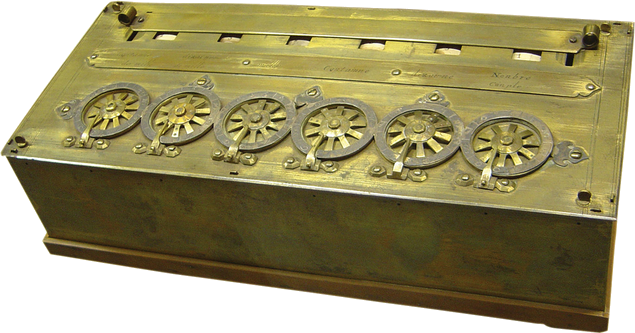
\includegraphics[width=.95\textwidth]{png/pascaline.png}

\textit{Pascaline -- 1652}

\end{center}
\end{minipage} \hfill
\begin{minipage}[c]{.24\linewidth}
\begin{center}
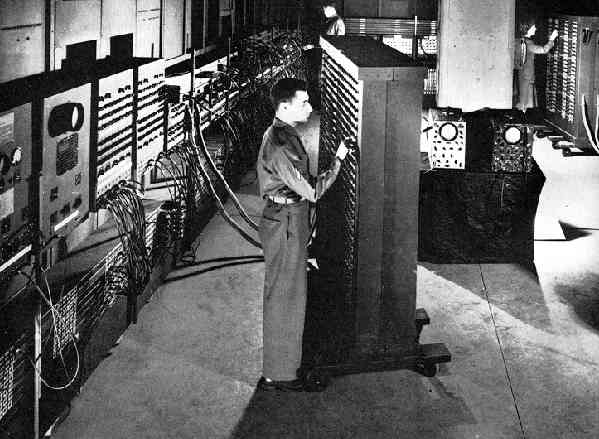
\includegraphics[width=.95\textwidth]{png/eniac.png}

\textit{ENIAC -- 1946}
\end{center}
\end{minipage} \hfill
\begin{minipage}[c]{.24\linewidth}
\begin{center}
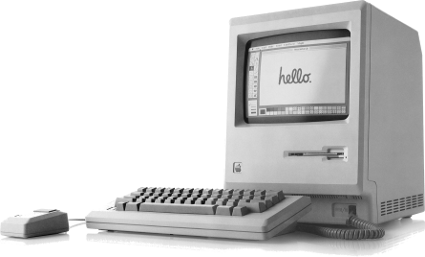
\includegraphics[width=.95\textwidth]{png/macintosh_p.png}

\textit{Macintosh -- 1984}
\end{center}
\end{minipage}\hfill
\begin{minipage}[c]{.24\linewidth}
\begin{center}
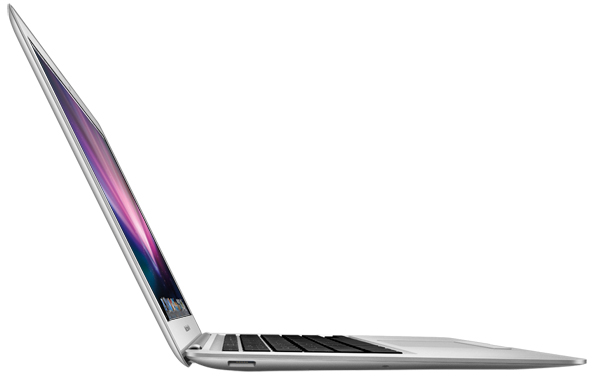
\includegraphics[width=.95\textwidth]{png/macbook.png}

\textit{MacBookAir -- 2008}
\end{center}
\end{minipage}

\vspace{.5cm}

\begin{Objectif}

\textsc{Savoir}
Dec - C1 :
\begin{itemize}
\item Se familiariser aux principaux composants d’une machine numérique telle que l’ordinateur personnel, une tablette, etc : sources d’énergie, mémoire vive, mémoire de masse, unité centrale, périphériques d’entrée-sortie, ports de communication avec d’autres composants numériques
\end{itemize}

\end{Objectif}


\setlength{\parskip}{0ex plus 0.2ex minus 0ex}
\renewcommand{\contentsname}{}
\renewcommand{\baselinestretch}{1}

\tableofcontents

\renewcommand{\baselinestretch}{1.2}
\setlength{\parskip}{2ex plus 0.5ex minus 0.2ex}


% \vspace{1cm}
\section{Architecture de base d'un ordinateur}
\subsection{Introduction}
L'informatique, contraction d'information et automatique, est la science du traitement de l'information. Apparue au milieu du 20ème siècle, elle a connu une évolution extrêmement rapide. À sa motivation initiale qui était de faciliter et d'accélérer le calcul, se sont ajoutées de nombreuses fonctionnalités, comme l'automatisation, le contrôle et la commande de processus, la communication ou le partage de l'information.
Ce cours expose les principes de base du traitement programmé de l’information. La mise en œuvre de ces systèmes s’appuie sur :
\begin{itemize}
\item le matériel (hardware), qui est l’objet de ce cours, correspond à l’aspect concret du système : unité centrale, mémoire, organes d’entrées-sorties, etc…
\item le logiciel (software) correspond à un ensemble d’instructions, appelé programme, qui sont contenues dans les différentes mémoires du système et qui définissent les actions effectuées par le matériel.
\end{itemize}


\subsection{Constitution d’un ordinateur du laboratoire}


\begin{figure}[H]
\begin{minipage}[c]{.49\linewidth}
\begin{center}
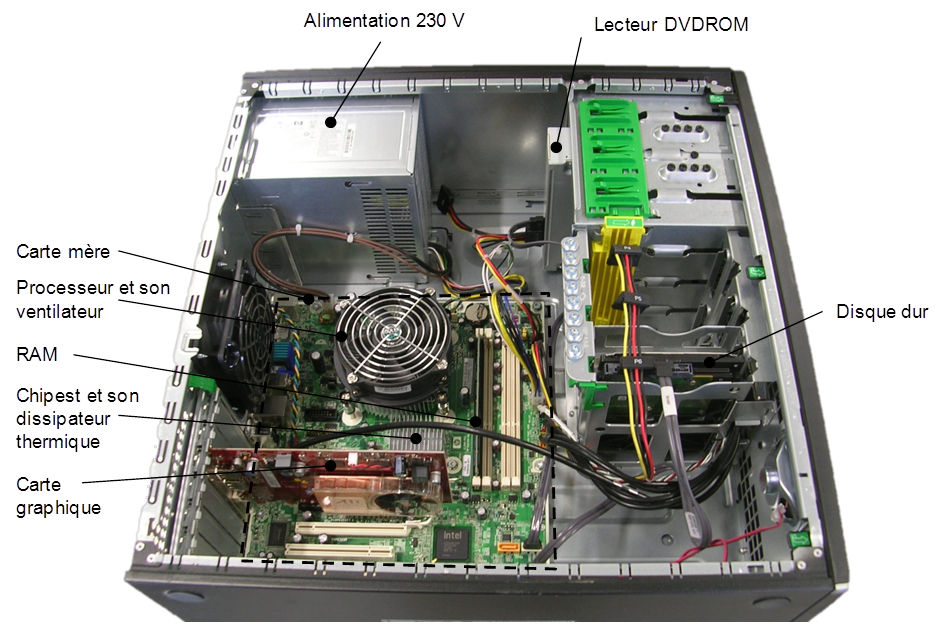
\includegraphics[width=.99\textwidth]{images/ordi1.png}
\label{}
\end{center}
\end{minipage} \hfill
\begin{minipage}[c]{.49\linewidth}
\begin{center}
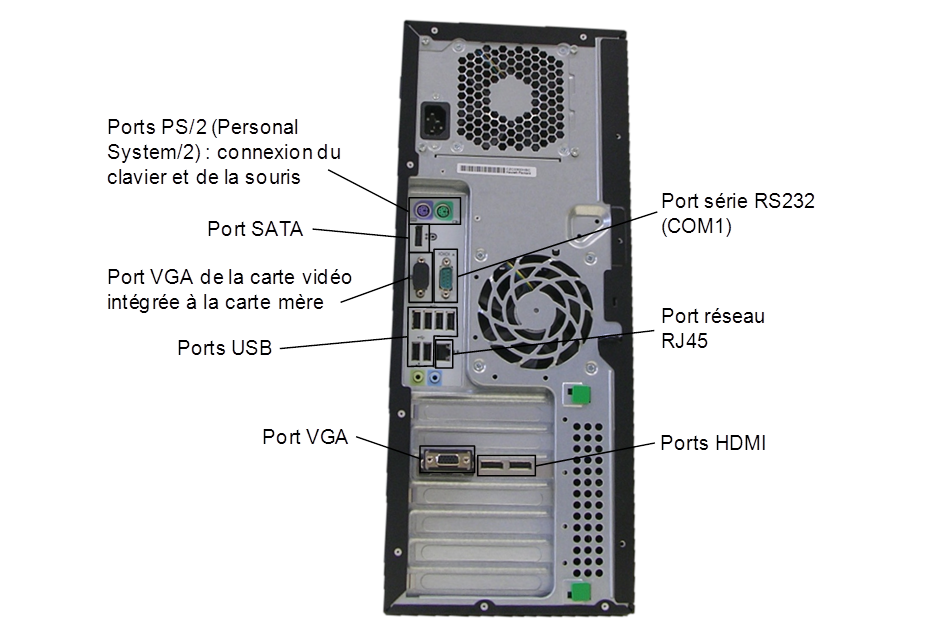
\includegraphics[width=.99\textwidth]{images/ordi2.png}
\label{}
\end{center}
\end{minipage}
\end{figure}

\subsection{Modèle de Von Neumann}

Pour pouvoir exécuter des algorithmes arbitraires, les ordinateurs actuels sont tous bâtis
autour du même modèle architectural théorique, l’architecture de Von Neumann, même
si la mise en oeuvre pratique est un peu plus complexe.

Le premier ordinateur électronique fut l’ENIAC
(dont le but était de calculer des tables indiquant les paramètres de tir d’une batterie d’artillerie
en fonction de la distance de l’objectif, du vent, etc.) dont la construction démarra
en 1943. 

\begin{figure}[H]
\begin{minipage}[c]{.49\linewidth}

Son architecture a été décrite dans un rapport de John Von Neumann en 1945 et
est depuis appelée «~architecture de Von Neumann~». Depuis près de 70 ans, à quelques variations
près, cette  architecture sert de base à la plupart des systèmes à microprocesseur actuel. Elle est composée des éléments suivants :
\begin{itemize}
\item d'une mémoire vive ;
\item d'un processeur qu'on peut conceptuellement décomposer en une unité de contrôle et
une unité de calcul arithmétique et logique ;
\item de dispositifs périphériques, appelés simplement périphériques ;
\item d'un canal de communication entre la mémoire, le processeur et les périphériques, appelé
le bus.
\end{itemize}

\end{minipage} \hfill
\begin{minipage}[c]{.49\linewidth}
\begin{center}
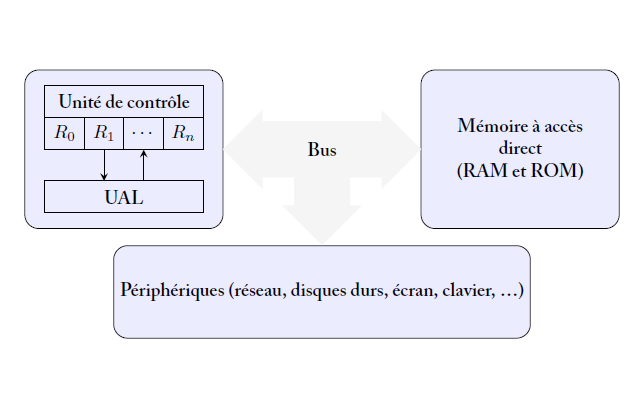
\includegraphics[width=.99\textwidth]{images/von.png}
\caption{Architecture de Von Neumann}
\label{}
\end{center}
\end{minipage}
\end{figure}




\section{La carte mère}
La carte mère constitue le c\oe{}ur d'un ordinateur. Elle est abritée par une tour sur un ordinateur de bureau ou par le boîtier sous le clavier dans un ordinateur portable. Elle est équipée de divers connecteurs permettant de brancher, l'alimentation, le(s) processeur(s)
les ventilateurs, 
la mémoire vive, 
le disque dur (et autres disques), 
la carte réseau, 
la carte son, 
la carte graphique lorsque celle-ci n'est pas intégrée, 
l(es)'écran(s), 
le clavier,  
la souris, 
les autres périphériques (imprimantes, scanner, lecteurs multimédias, téléphones ...).



\subsection{Cartes mères}

La plupart des cartes mères utilisées dans les ordinateurs de bureau sont au format ATX. Elles imposent donc certaines dimensions pour le boîtier (tour). Elles assurent la liaison avec tous les composants.

\begin{center}
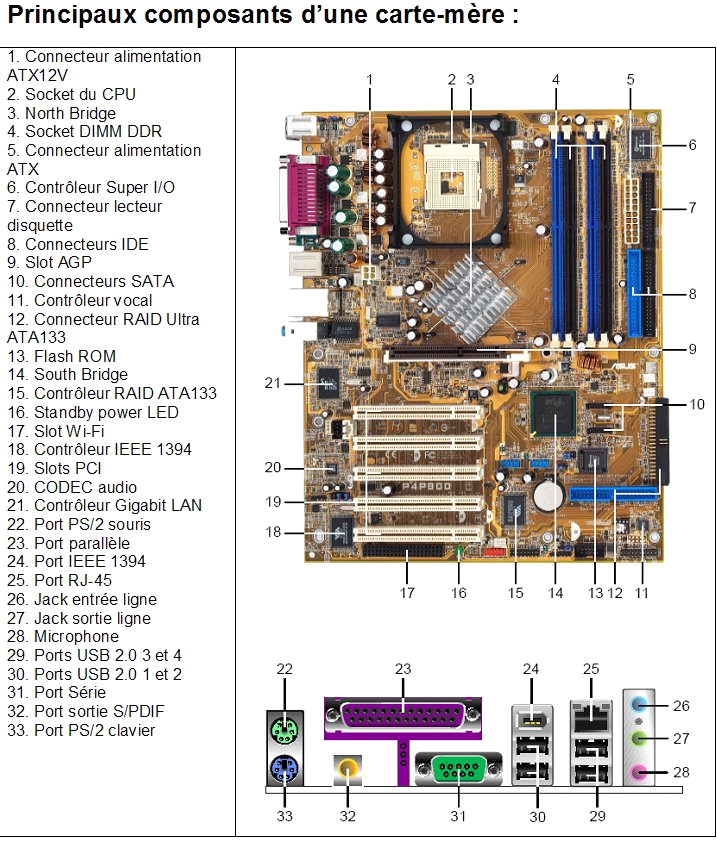
\includegraphics[width=.7\textwidth]{png/carte_mere_2.png}
\end{center}




\begin{figure}[H]
\begin{minipage}[c]{.49\linewidth}

Le fonctionnement de la carte mère est assuré par des chipsets (ensemble de composants électroniques) qui permettent l'échange des données entre les différents composants branchés. Le northbridge gère les composants branchés <<rapides>> (la mémoire cache par exemple). Le southbridge est le chipset permettant la gestion des composants <<lents>> (comme le disque dur). 

Le flux des informations est cadencé par une horloge permettant leur synchronisation. Cette horloge est alimentée de façon permanente par une pile. 

Le BIOS (\textit{Basic Input/Output System}) est un logiciel directement installé sur la carte mère qui permet d'assurer la communication entre le matériel et le système d'exploitation. 

\end{minipage} \hfill
\begin{minipage}[c]{.49\linewidth}
\begin{center}
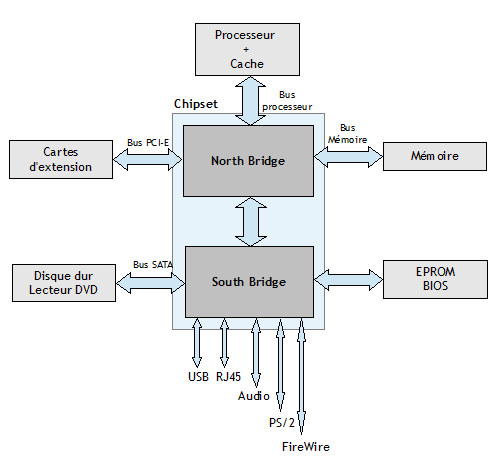
\includegraphics[width=.9\textwidth]{images/carte.png}
\label{}
\end{center}
\end{minipage}
\end{figure}

Sur la carte mère, la communication entre les différents composants est assurée par des bus :
\begin{itemize}
\item le bus système relie le micorprocesseur au chipset;
\item le bus mémoire relie le chipset à la mémoire vive;
\item le bus d'extension relie le chipset aux connecteurs d'entrée -- sortie.
\end{itemize}

\subsection{CPU (\textit{Central Processing Unit})}


\noindent\begin{minipage}[c]{.65\linewidth}
Le CPU aussi appelé processeur ou microprocesseur est le cerveau du PC. Sa puissance dépend du nombre de cœurs du processeur, de la taille de sa mémoire cache, de l'architecture du processeur et de sa fréquence.

La fréquence du CPU s'exprime en MHz ou en GHz. C'est une valeur à laquelle les utilisateurs
attachent le plus d'importance mais d'autres paramètres en déterminent les performances.
Dans un ordinateur, non seulement les données traitées sont discrètes, mais le déroulement
des opérations se fait aussi selon un temps discrétisé.
\end{minipage}\hfill
\begin{minipage}[c]{.3\linewidth}
\begin{center}
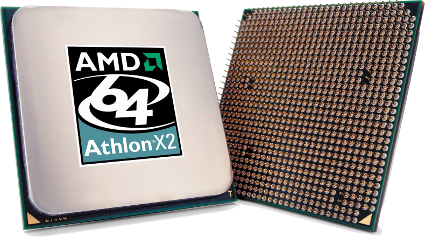
\includegraphics[width=.8\textwidth]{png/cpu_amd_p.png}
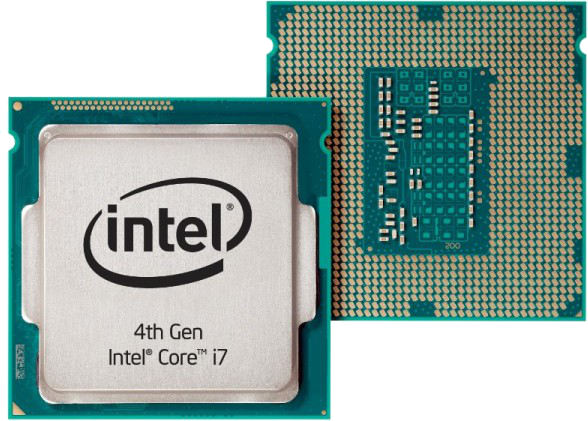
\includegraphics[width=.8\textwidth]{png/cpu_intel.png}
\end{center}
\end{minipage}

\vspace{.25cm}

La mémoire cache permet au processeur d'avoir à sa disposition une mémoire d'accès rapide mais dont la capacité est relativement limitée. 


Une horloge, le plus souvent calibrée à l'aide d'oscillateurs à quartz, émet régulièrement une suite d'impulsions, comme un métronome, qui sert à scander les opérations. Le temps d'un
cycle, ou période de l'horloge, est une caractéristique des processeurs : par exemple 1 Ghz,
c'est-à-dire une impulsion tous les milliardièmes de secondes.

L'efficacité du CPU dépend aussi de son architecture interne. Les processeurs actuels
traitent plusieurs instructions par cycle. Ces traitements se font en parallèle grâce
notamment à la technique du double pipeline d'instructions, ce qui leur permet d'effectuer
deux ou trois instructions par cycle.

Le rôle de la mémoire cache est d'autant plus important que la vitesse du CPU est élevée par
rapport à celle de la mémoire RAM. Cet écart ne cesse d'augmenter car l'évolution des CPU est bien plus rapide que celle des
mémoires. La mémoire cache coûte cher. Sa taille explique souvent la différence de prix
entre les processeurs.

L'augmentation des fréquences a atteint des limites aux environs de 4 GHz. La seule façon
d'augmenter encore les performances est maintenant de multiplier les cœurs sur la même
puce.


Un ensemble de fils appelé bus partent du CPU et permettent de le connecteur aux autres composants du système.
Le CPU est constitué essentiellement de trois parties :
\begin{itemize}
\item l'unité de commande qui cherche les instructions en mémoire, les décode et coordonne le
reste du processeur pour les exécuter. Une unité de commande élémentaire se compose
essentiellement d'un registre d'instruction et d'une unité <<décodeur / séquenceur>>;
\item l'Unité Arithmétique et Logique (UAL) exécute les instructions arithmétiques et logiques
demandées par l'unité de commande. Les instructions peuvent porter sur un ou plusieurs
opérandes. La vitesse d'exécution est optimale quand les opérandes se situent dans les
registres plutôt que dans la mémoire externe au processeur;
\item les registres sont des cellules mémoire interne au CPU. Ils sont peu nombreux mais d'accès
très rapide. Ils servent à stocker des variables, les résultats intermédiaires d'opérations
(arithmétiques ou logiques) ou encore des informations de contrôle du processeur.

\end{itemize}


\begin{center}
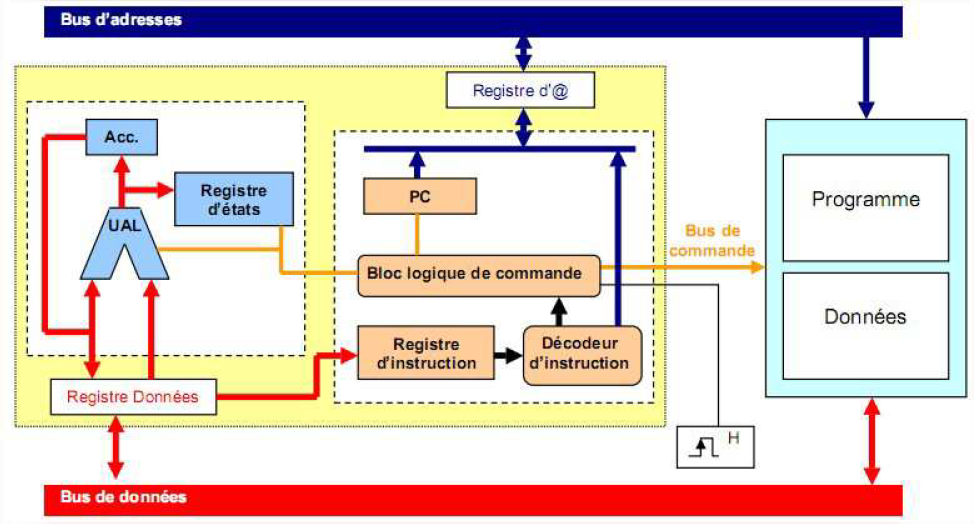
\includegraphics[width=.85\textwidth]{png/archi_cpu}
\end{center}

La structure des registres varie d'un processeur à l'autre. C'est ce qui fait que chaque type de CPU a un jeu d'instruction qui lui est propre. Leurs fonctions de base sont néanmoins
semblables et tous les processeurs possèdent en gros les mêmes catégories de registres :
\begin{itemize}
\item l'accumulateur est principalement destiné à contenir les données qui doivent être
traitées par l'UAL;
\item les registres généraux servent au stockage de résultats intermédiaires;
\item les registres d’adresse servent à confectionner des adresses de données
particulières : ce sont, par exemples, les registres de base et d'index qui permettent
entre autres d'organiser les données en mémoire comme des tables indicées.
\item le registre d'instruction (RI) contient le code de l'instruction qui est traitée par le
décodeur / séquenceur;
\item le compteur ordinal (CO) ou Program Counter (PC) contient l'adresse de la
prochaine instruction à exécuter. En principe, ce registre ne cesse de compter. Il
génère les adresses des instructions à exécuter les unes à la suite des autres.
Certaines instructions demandent quelquefois de changer le contenu du compteur
ordinal pour faire une rupture de séquence c'est à dire un saut ailleurs dans le
programme.
\end{itemize}


\subsection{Les bus}

En informatique, le terme bus désigne un ensemble de fils support de l'information et organe de communication entre différents composants.Il existe deux grands types de bus :
\begin{itemize}
\item le bus série : il comporte plusieurs fils, dont la masse (référence de potentiel), le fil de données, le fil d'horloge. Les données sont transmises en série;
\item le bus parallèle : il comporte un fil de masse, un fil d'horloge, et $n$ fils de données pour un bus $n$ bits ; les données sont transmises en parallèle.
\end{itemize}

Par ailleurs, des bus sont intégrés dans des puces. Par exemple, dans les microprocesseurs, les différents constituants communiquent entre eux par des bus parallèles.
	
Sur la carte mère sont intégrés différents bus parallèles que l'on peut même parfois distinguer. Ces bus permettent de relier les différents constituants entre eux afin qu'ils communiquent. On retrouve des bus d'adresses, de données et de contrôle.

Entre la carte mère et les différents périphériques (disque dur par exemple), on utilise de plus en plus des bus séries. Ainsi, après le tout IDE, bus parallèle qui a été massivement utilisé dans les ordinateurs grand public, le bus SATA est de plus en plus utilisé. .

Le bus SATA ou S-ATA (\textit{Serial ATA}) a été conçu afin de pallier aux problèmes constatés à haute fréquence sur le bus IDE encore appelé Parallel ATA.
Plusieurs normes SATA ont été développées. 

\begin{center}
\begin{tabular}{|c|c|}
\hline
Norme & Débit ($Mo/s$) \\
\hline
SATA I & 187,5 \\ \hline
SATA II & 375 \\ \hline
SATA III & 750 \\ \hline
\end{tabular}
\end{center}

Cette technologie présente des débits bien plus importants que les disques durs mécaniques  (60 Mo/s au mieux) mais va en revanche bien s'adapter aux débits des SSD qui commencent à avoisiner les 500 Mo/s.


\section{Les mémoires}
\subsection{Mémoire de masse}
\subsubsection{Le disque-dur magnétique}


\paragraph*{Description}
\begin{minipage}[c]{.65\linewidth}
Le disque dur (\textit{HDD -- Hard Disk Drive}) doit son nom à sa technologie à l'époque où existaient encore les disques souples, ou disquettes.

Le disque dur est alimenté par un connecteur Molex ou par adaptateur de courant SATA. Ces connecteurs sont reliés à l'alimentation du PC. 

La capacité des disques durs actuels atteint les 4 To (téraoctet). Lorsqu'ils sont connectés en SATA, le débit oscille entre 30 et 60 \textit{Mo/s} et peut atteindre les 600 \textit{Mo/s}. Enfin, pour améliorer les performances d'accès aux données, ils possèdent une mémoire cache pouvant aller jusqu'à 128 \textit{Mo} sur laquelle sont stockées les informations fréquemment utilisées. 

\end{minipage}\hfill
\begin{minipage}[c]{.3\linewidth}
\begin{center}
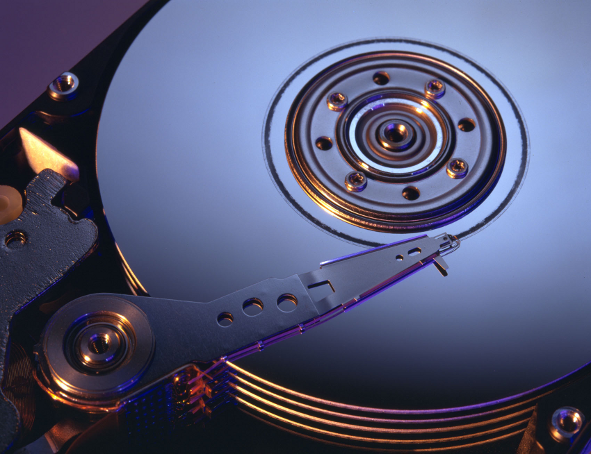
\includegraphics[width=.7\textwidth]{png/dd_1_p.png}
\end{center}
\end{minipage}


\paragraph*{Principe de fonctionnement}


\begin{minipage}[c]{.6\linewidth}
Un disque dur est composé de disques rigides et paramagnétiques (en aluminium, en verre ou en céramique) recouverts d'une couche magnétique et d'un film protecteur. Ces plateaux sont entraînés par un moteur électrique dont la fréquence de rotation est fixe. La fréquence de rotation peut atteindre les 15 000 \textit{tr/min}. Un bras, sur lequel sont fixées les têtes de lecture -- écriture, est aussi motorisé pour atteindre les différentes parties du disque. La distance entre les têtes et les plateaux est de l'ordre de 10 \textit{nm}. Elle est maintenue par un coussin d'air formé par la rotation des disques. 
\end{minipage} \hfill
\begin{minipage}[c]{.35\linewidth}
\begin{center}
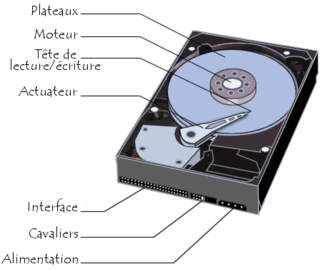
\includegraphics[width=.9\textwidth]{png/dd_comp.png}
\end{center}
\end{minipage} 

Les têtes de lecture -- écriture sont inductives et permettent de générer un champ magnétique dans deux sens opposés permettant de polariser la couche magnétique du disque. Ainsi, en mode lecture les changements de polarité sont transcrits par un convertisseur analogique numérique (CAN) en bits (0 ou 1).

Les données sont organisées en pistes concentriques, les données les plus rapidement accessibles étant celles situées sur le disque extérieur. Chaque piste est divisée en secteurs (d'un minimum de 512 octets). Enfin, on appelle cylindre l'ensemble de données situé sur une même piste mais sur un plateau différent. 


%
%\begin{center}
%\begin{tabular}{|c|c|c|c|c|}
%\hline
%Capacité & Année & Fabriquant & Modèle & Taille \\ \hline
%5 Mo & 1956 & IBM & 305 RAMAC & 24''\\ \hline
%28 Mo & 1962 & IBM & Modèle 1301 & \\ \hline
%1.02 Go & 1982 & Hitachi & H8598 & 14''\\ \hline
%25 Go & 1998 & IBM & Deskstar 25 GP & 7,0'' \\ \hline
%500 Go & 2005 & Hitachi & & 3,5''\\ \hline
%1 To & 2007 & Hitachi & Deskstar 7K1000 & 3,5''\\ \hline
%2 To & 2009 & Western Digital & Caviar Green WD20EADS & 3,5''\\ \hline
%3 To & 2010 & Seagate & & 3,5''\\ \hline
%4 To & 2011 & Hitachi & 7K4000 & 3,5''\\
%\hline
%\end{tabular}
%
%\textit{Capacité actuelle des ordinateurs}
%\end{center}





\subsubsection{Disques dur SSD -- \textit{Solid State Drive}}




\begin{center}
\begin{tabular}{|l|l|l|}
\hline
\textbf{Caractéristiques} & \textbf{Disque dur mécanique} & \textbf{SSD} \\ \hline
Temps d'accès & En moyenne 12ms & 0.1ms \\ \hline
Poids & De 400g à 700g & Quelques dizaines de grammes \\ \hline
Consommation en veille & De l'ordre du Watt & 100 mW \\ \hline
Consommation en activité & 4W environ & 900 mW \\ \hline
Bruit  & En moyenne 40 dB & 0 dB\\ \hline
\end{tabular}
\end{center}

Les performances du SSD sont supérieures à celles des disques durs classiques. Deux critères penchent néanmoins en sa défaveur. D'une part le prix du Go est presque 10 fois plus élevé 
que pour un disque dur mécanique. D'autre part, certaines technologies de SSD présentent l'inconvénient d'être limité en nombre de cycles d'écriture -- lecture.

\subsubsection{Disques durs hybrides}
Le disque dur hybride est l'exact compromis entre un disque dur mécanique « conventionnel » et un disque dur SSD. C'est un disque dur mécanique auquel on a adjoint un volume mémoire flash conséquent (quelques Go), ou du moins suffisant pour que l'effet s'en ressente sur son utilisation en comparaison d'un disque dur mécanique. L'intérêt est une réduction très nette du prix du disque dur pour des performances accrues tout en limitant les risques de pertes de mémoire sur le SSD de technologie encore limitée en nombre de cycles mémoires.


Actuellement, l'un des disques de plus grande capacité est le Seagate Momentus XT 7200 Hybrid SSD 750Go SLC 8Go NAND Flash. On trouve également dans la marque Western Digital le WD Black SSHD, 1 To en stockage classique et 24 Go de mémoire NAND Flash.



\subsection{La mémoire vive}

\noindent \begin{minipage}[c]{.6\linewidth}
Les mémoires de type RAM (\textit{Random Access Memory} -- Mémoire à accès aléatoire) sont des mémoires dites volatiles, c'est-à-dire dont le contenu disparaît en absence d'alimentation.
Elles sont utilisées bien-sûr dans les PC et autres ordinateurs personnels comme mémoire de travail du système. Les mémoires Cache sont également des RAM.


\end{minipage}
\begin{minipage}[c]{.3\linewidth}
\begin{center}
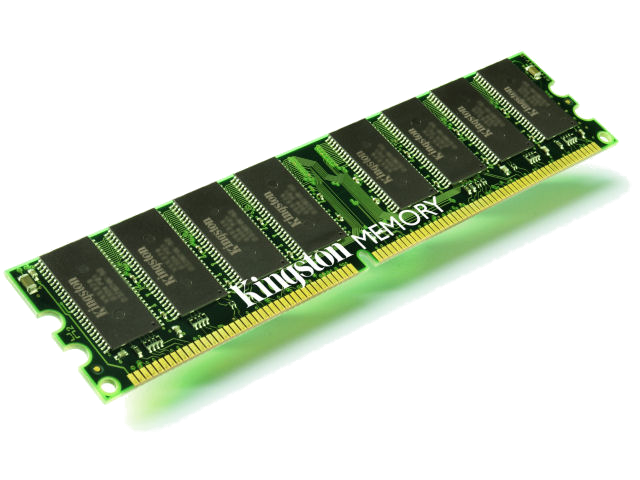
\includegraphics[width=.9\textwidth]{png/ram.png}
\end{center}
\end{minipage}

Une autre grosse différence avec les ROM concerne la fréquence de fonctionnement (ou le temps d'accès) des RAM. La fréquence de fonctionnement de la RAM en général est beaucoup plus élevée que pour la ROM. La raison principale en est une différence essentielle de structure.

Le temps d'accès des mémoires RAM est de quelques nanosecondes pour une capacité de l'ordre de quelques Go.


\subsection{La mémoire ROM (« mémoire morte »)}


\begin{figure}[H]
\begin{minipage}[c]{.49\linewidth}

Historiquement, les ROM (\textit{Read Only Memory}-- Mémoire en lecture seule) étaient effectivement des mémoires en lecture seule. Leur grosse différence avec les RAM est que leur contenu perdure malgré l'absence d'alimentation. Elles seront donc par exemple très utiles pour stocker les programmes et informations de démarrage (BIOS, Setup CMOS, le POST (Power On Self Test)). Mais leurs fonctions ne se limitent pas à celle-ci.

\end{minipage} \hfill
\begin{minipage}[c]{.49\linewidth}
\begin{center}
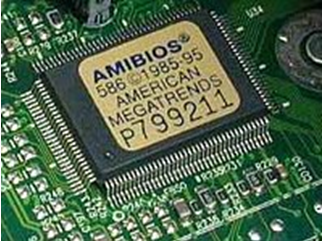
\includegraphics[width=.5\textwidth]{images/ROM.png}
\label{}
\end{center}
\end{minipage}
\end{figure}
Actuellement, on utilise le plus souvent des EEPROM ( Electrically Erasable Programmable ROM ).

Si l'appellation ROM désigne le plus souvent les puces mémoires, on ne peut oublier :
\begin{itemize}
\item les CD-ROM, les DVD-ROM
\item les Bluray sont des ROM
\item les disques durs sont des ROM ( car non volatiles )
\item les SSD sont des ROM
\item les clefs USB sont des ROM ( mémoire flash )
\end{itemize}

Le temps d'accès pour une puce ROM du type de celles utilisées pour le BIOS ou la CMOS est de l'ordre de quelques dizaine de nanosecondes. Leur capacité varie selon le support considéré (puce, SSD, \textit{etc.}).


\section{Communication}

\subsection{Connectique}
\subsubsection{Le port USB \cite{usb}}

\noindent \begin{minipage}[c]{.75\linewidth}
USB (\textit{Universal Serial Bus} -- bus série universel) est un protocole de communication apparu en 1996 (USB 1.0). Ce protocole série a révolutionné les connexions entre PC et périphériques en instaurant un environnement « tout USB », uniformisant les modes de communication avec l'ordinateur... C'est sans doute le bus de communication le plus utilisé. Ses principaux concurrents sont désormais les protocoles sans fil Bluetooth et WiFi.
\end{minipage}\hfill
\begin{minipage}[c]{.2\linewidth}
\begin{center}
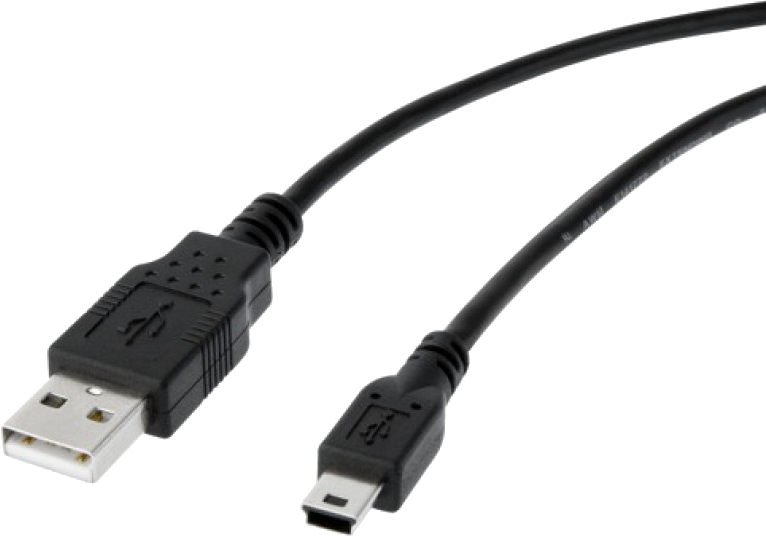
\includegraphics[width=\textwidth]{png/usb.png}
\end{center}
\end{minipage}

\begin{center}
\begin{tabular}{|l|l|l|l|l|}
\hline
Version & USB 1.0 & USB 1.1 & USB 2.0 & USB 3.0 \\ \hline
Débit   & 0,19 $Mo/s$ & 1,5 $Mo/s$ & 60 $Mo/s$ & 600 $Mo/s$  \\ \hline
\end{tabular}
\end{center}

Un connecteur USB est composé de 4 fils : 
\begin{itemize}
\item un fil d'alimentation (5V -- VBUS);
\item un fil de masse (GND);
\item deux fils de données (D+ et D- torsadés). 
\end{itemize}

Afin de faire transiter l'information, l'USB utilise des paquets. Ainsi une transaction USB est composée de 3 paquets :
\begin{itemize}
\item le paquet \textit{token} contient des informations sur la nature de la communication (est-ce l'hôte ou le périphérique qui envoie de l'information ?);
\item le paquet de données;
\item le paquet \textit{handshake} qui contient des informations sur le déroulement de la transaction (le paquet a été reçu correctement, interruptions lors de la transaction...).
\end{itemize}


\subsubsection{Le port série}

Pour les communications séries, les connecteurs sont de type D-SUB (DB9 par exemple).

Historiquement, le port série est le premier port de communication utilisant une transmission série (norme RS232). Son débit est au maximum de 19200 bps (bits par seconde). Il a été très longtemps utilisé pour sa simplicité de configuration et de pilotage. C'est d'ailleurs le protocole de communication mis en œuvre pour un grand nombre de système du laboratoire : MAXPID, cordeuse, DAE, etc. A noter cependant que si certains PC ont encore un port COM1 RS232, la plupart utilise un adaptateur RS232-USB pour communiquer avec le PC.

\subsubsection{Le port parallèle}
Pour les communications séries, les connecteurs sont de type D-SUB (DB25 par exemple).

Le port parallèle est un port reposant sur un protocole unidirectionnel de communication parallèle. Il est en voie d'extinction, comme le port série RS232. Il était le plus souvent utilisé pour la communication PC--imprimante. Le débit maximum  est de 16Mbps.


\subsubsection{Port PS/2 -- \textit{Personal System/2}}

\begin{minipage}[c]{.75\linewidth}
Le port PS/2 utilise un connecteur mini-din. 
Ce port de communication de taille réduite a succédé au PS/1 (Din, le même en plus encombrant ) permettant la connexion du clavier et/ou de la souris créé par IBM (1987) mais démocratisé en 1995 suite à son intégration sur les cartes mères type ATX. 

Il est également supplanté par le standard USB depuis quelques années mais également de plus en plus par le bluetooth.
\end{minipage}\hfill
\begin{minipage}[c]{.2\linewidth}
\begin{center}
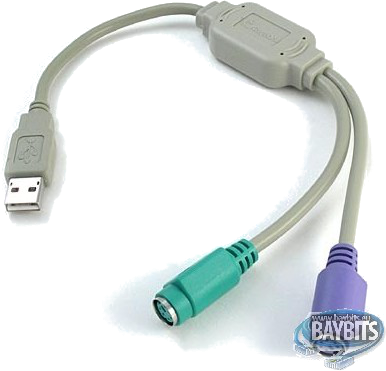
\includegraphics[width=\textwidth]{png/ps2.png}
\end{center}
\end{minipage}


\subsection{Communication réseau}
\subsubsection{Port RJ45 -- \textit{Registered Jack}}

\begin{minipage}[c]{.7\linewidth}
Ce port permet la connexion filaire réseau ethernet (LAN : Local Area Network) par câble. Différents protocoles existent, spécifiant différents débits.

\begin{center}
\begin{tabular}{|c|c|c|c|}
\hline
Protocole & Gigabits & 10GBase-X & 100GBase-X \\ \hline
Débit & 128 Mo/s & 1280 Mo/s & 12 800 Mo/s\\ \hline
\end{tabular}
\end{center}


\end{minipage}\hfill
\begin{minipage}[c]{.25\linewidth}
\begin{center}
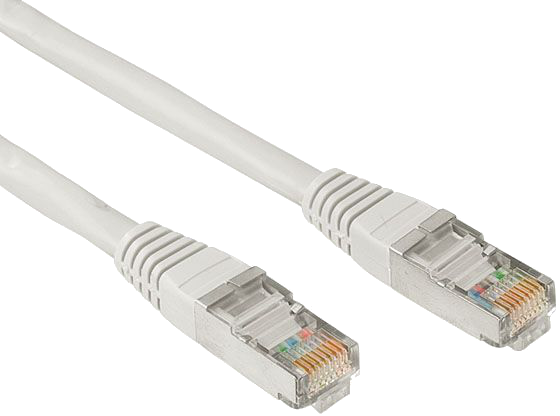
\includegraphics[width=.9\textwidth]{png/ethernet.png}
\end{center}
\end{minipage}\hfill



\subsubsection{Wi-Fi}

Le Wi-Fi (\textit{Wireless Fidelity} -- Norme \textit{IEEE 802.11}) est un standard définissant les caractéristiques d'un réseau local sans fil. La liaison est assurée par l'intermédiaire d'ondes électromagnétiques.  

Différentes normes physiques définissent le débit de la transmission en fonction de la portée. 
\begin{center}
\begin{tabular}{|c|c|c|c|}
\hline
\textbf{Standard} & \textbf{Bande de fréquence} & \textbf{Débit} & \textbf{Portée} \\ \hline
WiFi a (802.11a) & 5 GHz & 54 Mbit/s & 10 m \\ \hline
WiFi B (802.11b) & 2,4 GHz -- 2,5 GHz& 11 Mbit/s & 100 m \\ \hline
WiFi G (802.11g) & 2,4 GHz -- 2,5 GHz & 54 Mbit/s & 75 m \\ \hline
WiFi N (802.11n) & 2,4 GHz ou 5 & 450 Mbit/s & 125 m \\ \hline
\end{tabular}
\end{center}


\subsubsection{3G -- 4G}
La 3G et la 4G sont les troisième et les quatrième générations de transmissions de données pour la téléphonie mobile. La 4G permet d'avoir accès à des débits théoriques très supérieurs à la 3G et possède un c\oe{}ur de réseau basé sur IP. 

\textit{Tableau récapitulatif \url{http://www.commentcamarche.net/}}
\begin{center}
\begin{tabular}{|c|c|p{6cm}|c|c|}
\hline
Standard	& Génération	&Bande de fréquence	& Débit & \\
\hline 
GSM	& 2G & Permet le transfert de voix ou de données numériques de faible volume.&	9,6 kpbs	&9,6  kpbs \\ \hline
GPRS &2.5G & Permet le transfert de voix ou de données numériques de volume modéré.&	21,4-171,2 kpbs	&48 kpbs \\ \hline
EDGE & 2.75G & 	Permet le transfert simultanés de voix et de données numériques.&	43,2-345,6 kbps&	171 kbps \\ \hline
UMTS & 3G &Permet le transfert simultanés de voix et de données numériques à haut débit.&	0.144-2 Mbps	&384 Kbps \\ \hline
LTE & 4G	& Permet le transfert simultanés de voix et de données numériques à haut débit.&	10-300 Mbps	&5-75 Mbps \\ \hline
\end{tabular}
\end{center}

\subsection{Son et vidéo}




\begin{minipage}[c]{.85\linewidth}
Le port VGA -- \textit{Video Graphics Array}

Le connecteur est de type D-SUB, ici DE-15. Ce port est de type analogique.

\end{minipage} \hfill
\begin{minipage}[c]{.14\linewidth}
\begin{center}
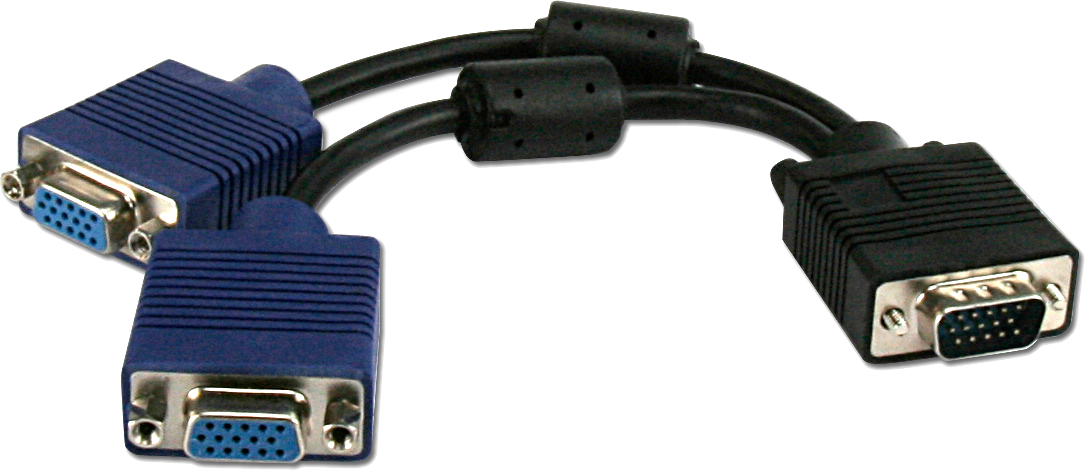
\includegraphics[width=.9\linewidth]{png/vga}
\end{center}
\end{minipage}


\begin{minipage}[c]{.85\linewidth}
Le port DVI -- \textit{Digital Visual Interface}

Ce port est de type numérique non HD. Il apporte une amélioration en terme de réduction du bruit par rapport au connecteur VGA analogique.
\end{minipage} \hfill
\begin{minipage}[c]{.14\linewidth}
\begin{center}
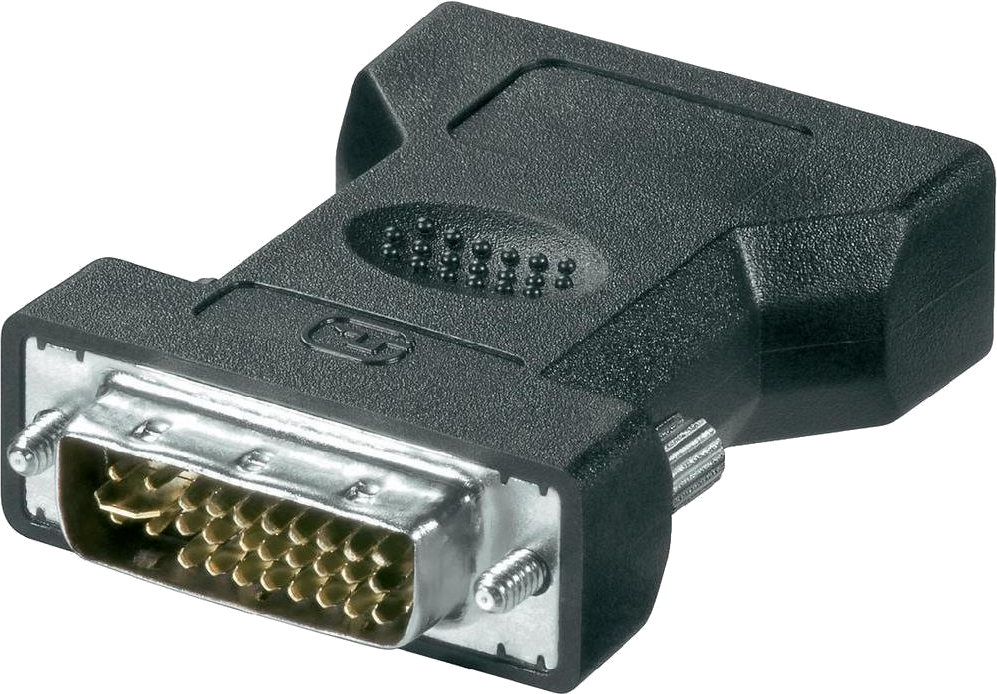
\includegraphics[width=.9\linewidth]{png/dvi}
\end{center}
\end{minipage}


\begin{minipage}[c]{.85\linewidth}
Le port HDMI -- \textit{High Definition Multimedia Interface}

Il s'agit d'une interface audio vidéo totalement numérique permettant de raccorder un lecteur de disque, une console, un décodeur \textit{etc.} à un écran de télévision haute définition.
\end{minipage} \hfill
\begin{minipage}[c]{.14\linewidth}
\begin{center}
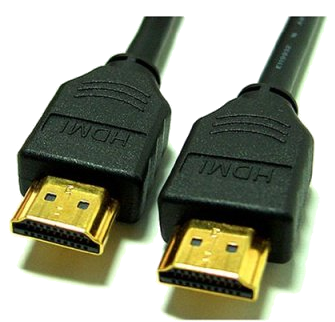
\includegraphics[width=.9\linewidth]{png/hdmi}
\end{center}
\end{minipage}




\footnotesize

\begin{thebibliography}{2}
\bibitem{medevielle}{François Médevielle, Architecture des ordinateurs -- UPSTI}
\bibitem{beynet}{Patrick Beynet, ISN -- Architectures matérielles -- Architecture des ordinateurs. Lycée Rouvière.}

\bibitem{wikipedia}{\url{http://fr.wikipedia.org/wiki/Disque_dur}.}
\bibitem{ccm}{\url{http://www.commentcamarche.net/contents/740-disque-dur}.}

\bibitem{cm}{Carte mère. \url{http://micropuces-informatique.fr/?page_id=29}}
\bibitem{ram}{\url{http://nouvelleteckno.files.wordpress.com/2011/11/ddr.jpg}}
\bibitem{dd1}{\url{http://www.builttoordercomputers.com/wp-content/uploads/2011/04/Hard-Disk-Drive-1.jpg}}
\bibitem{dd2}{\url{http://www.reviversoft.com/blog/wp-content/uploads/2013/01/hard_drive_problems_harddrive_02.jpg}}
\bibitem{dd_ssd}{\url{http://www.militarysystems-tech.com/files/militarysystems/imagecache/Original/supplier_images/Solid\%20State\%20Drive\%20SSD\%20Galatea\%20100GB\%20200GB\%20Encryption-l.jpg}}
\bibitem{usb}{\url{http://fr.ids-imaging.com/store/media/catalog/product/cache/4/image/795x795/9df78eab33525d08d6e5fb8d27136e95/u/s/usb2_cable_standard_2.jpg}}
\bibitem{ps2}{\url{http://www.baybits.eu/174-607-thickbox/adaptateur-convertisseur-usb-ps2-ps-2-clavier-et-souris.jpg}}
\bibitem{ethernet}{\url{http://brain.pan.e-merchant.com/2/4/46000142/l_46000142.jpg}}
\bibitem{cm2}{Carte mère. \url{http://serveurfelix.myds.me/~Felix/HTTrack/doku505c.html?id=architecture_pc:architecture_pc:composants}}
\bibitem{usb}{\url{http://u.s.b.free.fr/pdf/L_USB_et_sa_norme_v1.pdf}}
\end{thebibliography}

 


\end{document}